\documentclass{article}
\usepackage[english]{babel}
\usepackage{meta-inf/lib/naproche}
\documentclass[12pt,oneside]{book}

\usepackage[foundations]{../../lib/tex/naproche}
\usepackage{../../lib/tex/libraries}
\usepackage{graphicx}
\usepackage{float}
\usepackage{caption}
\usepackage{footnote}

\makesavenoteenv{tabular} % Make footnotes work in tabular environments


\title{Foundations of Mathematics}
\author{Marcel Schütz}
\date{2022}

\begin{document}
  \maketitle

  \tableofcontents

  \begin{figure}[H]
    \centering
    \fbox{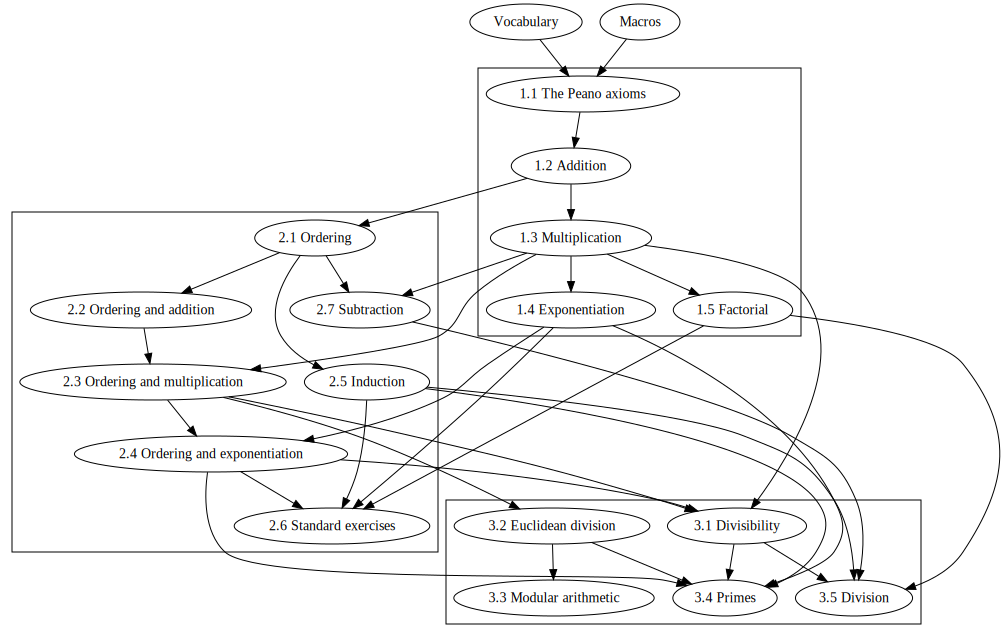
\includegraphics[width=0.9\linewidth]{./dependency-graph/graph.png}}
    \caption*{Interdependencies of the chapters}
  \end{figure}


  \section*{Introduction}

  This is a library providing a foundation of mathematics based on a
  Kelley-Morse like class theory with urelements.
  It introduces common operations on classes like unions or intersections
  (\cref{chapter:classes}) together with detailed proofs of their algebraic
  properties (\cref{chapter:computation-laws-for-classes}), the symmetric
  difference of two classes (\cref{chapter:symmetric-difference}) and the
  notions of ordered pairs and Cartesian products
  (\cref{chapter:pairs-and-products}) as well as proofs of the algebraic
  properties of the latter (\cref{chapter:computation-laws-for-products}).
  Moreover, it provides common operations on maps (\cref{chapter:maps}), various
  properties of images and preimages (\cref{chapter:image-and-preimage}) and the
  notions of injectivity, surjectivity, bijectivity
  (\cref{chapter:injections-surjections-bijections}) and invertibility of maps
  (\cref{chapter:invertible-maps}).
  The library provides an axiom system characterizing sets (\cref{chapter:sets})
  and, furthermore, it covers the notions of binary relations
  (\cref{chapter:binary-relations}), fixed-points of subset preserving maps
  (\cref{chapter:fixed-points}), including and equinumerosity
  (\cref{chapter:equinumerosity}).

  As two famous results it includes the Knaster-Tarski fixed point theorem
  (\cref{FOUNDATIONS_12_8420450166112256}) and the Cantor-Schröder-Bernstein
  theorem (\cref{FOUNDATIONS_13_1913663275401216}).

  \paragraph*{Usage.}
  At the very beginning of each chapter you can find the name of its source
  file, e.g. \path{foundations/sections/01_classes.ftl.tex} for
  \cref{chapter:classes}. This filename can be used to import the chapter via
  \Naproche's \texttt{readtex} instruction to another ForTheL text, e.g.:
  \begin{center}
    \verb`[readtex \path{foundations/sections/01_classes.ftl.tex}]`
  \end{center}

  \paragraph*{Checking times.}
  The checking times for each of the chapters may vary from computer to
  computer, but on mid-range hardware they are likely to be similar to those
  given in table below:

  \begin{center}
    \begin{tabular}{c|c|c}

      & \multicolumn{2}{c}{\textbf{Checking time}}
      \\
      \textbf{Chapter}
      & \textbf{without dependencies}     & \textbf{with dependencies}
      \\ \hline
      \ref{chapter:classes}
      & 00:04 min                         & 00:04 min
      \\
      \ref{chapter:computation-laws-for-classes}
      & 00:12 min                         & 00:16 min
      \\
      \ref{chapter:symmetric-difference}
      & 00:32 min                         & 00:48 min
      \\
      \ref{chapter:pairs-and-products}
      & 00:08 min                         & 00:12 min
      \\
      \ref{chapter:computation-laws-for-products}
      & 01:36 min                         & 01:56 min
      \\
      \ref{chapter:maps}
      & 01:13 min                         & 01:25 min
      \\
      \ref{chapter:image-and-preimage}
      & 01:28 min                         & 02:53 min
      \\
      \ref{chapter:injections-surjections-bijections}
      & 00:38 min                         & 02:03 min
      \\
      \ref{chapter:invertible-maps}
      & 02:20 min                         & 04:23 min
      \\
      \ref{chapter:sets}
      & 02:17 min                         & 06:40 min
      \\
      \ref{chapter:binary-relations}
      & 00:14 min                         & 06:54 min
      \\
      \ref{chapter:fixed-points}
      & 00:33 min                         & 07:13 min
      \\
      \ref{chapter:equinumerosity}
      & 01:48 min                         & 09:01 min
    \end{tabular}
  \end{center}


  \subfile{sections/01_classes.ftl.tex}
  \subfile{sections/02_computation-laws-for-classes.ftl.tex}
  \subfile{sections/03_symmetric-difference.ftl.tex}
  \subfile{sections/04_pairs-and-products.ftl.tex}
  \subfile{sections/05_computation-laws-for-products.ftl.tex}
  \subfile{sections/06_maps.ftl.tex}
  \subfile{sections/07_image-and-preimage.ftl.tex}
  \subfile{sections/08_injections-surjections-bijections.ftl.tex}
  \subfile{sections/09_invertible-maps.ftl.tex}
  \subfile{sections/10_sets.ftl.tex}
  \subfile{sections/11_binary-relations.ftl.tex}
  \subfile{sections/12_fixed-points.ftl.tex}
  \subfile{sections/13_equinumerosity.ftl.tex}
\end{document}

\usepackage{amssymb}

\newcommand{\Nat}{\mathbb{N}}
\newcommand{\Prime}{\mathbb{P}}
\renewcommand{\succ}{\textrm{succ}}
\newcommand{\pred}{\textrm{pred}}
\newcommand{\add}{\textrm{add}}
\newcommand{\mul}{\textrm{mul}}
\renewcommand{\exp}{\textrm{exp}}
\newcommand{\fac}{\textrm{fac}}
\renewcommand{\div}{\mathop{\textrm{div}}}
\renewcommand{\mod}{\mathop{\textrm{mod}}}


\usepackage[
  type=CC,
  modifier=by-nc-sa,
  version=4.0,
]{doclicense}

\newcommand{\gauss}{\mathcal{G}}

\title{Little Gauß' Theorem}
\author{\Naproche formalization: \vspace{0.5em} \\
Christian Schöner, Marcel Schütz}
\date{2024}

\begin{document}
  \pagenumbering{gobble}
  \maketitle

  \begin{imports}
    \begin{forthel}
      %[prove off][check off]
      [readtex \path{libraries/source/arithmetics/multiplication.ftl.tex}]
      %[prove on][check on]
    \end{forthel}
  \end{imports}

  \noindent This is a formalization of ``Little Gauß' Theorem'', i.e. of
  the assertion that
  \[\sum_{k=0}^n k = \frac{k(k + 1)}2\]
  for all $n \in \Nat$.
  In \Naproche we can define the sum $\sum_{n=0}^k n$ by the function
  $\gauss : \Nat \to \Nat$ with $\gauss(0) = 0$ and
  $\gauss(n + 1) = \gauss(n) + (n + 1)$:

  \begin{forthel}
    \begin{signature*}
      Let $n$ be a natural number.
      $\gauss(n)$ is a natural number.
    \end{signature*}

    \begin{axiom*}
      $\gauss(0) = 0$.
    \end{axiom*}

    \begin{axiom*}
      Let $n$ be a natural number.
      Then $\gauss(n + 1) = \gauss(n) + (n + 1)$.
    \end{axiom*}
  \end{forthel}

  \noindent Then the theorem can be stated as follows.

  \begin{forthel}
    \begin{theorem*}[Little Gauß]\label{little_gauss}
      For all natural numbers $n$ we have
      \[2 \cdot \gauss(n) = n \cdot (n + 1).\]
    \end{theorem*}
    \begin{proof}
      Define $\Phi = \{n \in \Nat \mid 2 \cdot \gauss(n) = n \cdot (n + 1)\}$.

      (1) $0 \in \Phi$.

      (2) For all $n \in \Phi$ we have $n + 1 \in \Phi$.\\
      Proof.
        Let $n \in \Phi$.
        Then $2 \cdot \gauss(n) = n \cdot (n + 1)$.
        Hence $2 \cdot \gauss(n + 1)
          = 2 \cdot (\gauss(n) + (n + 1))
          = (2 \cdot \gauss(n)) + (2 \cdot (n + 1))
          = (n \cdot (n + 1)) + (2 \cdot (n + 1))
          = ((n + 1) \cdot n) + ((n + 1) \cdot 2)
          = (n + 1) \cdot (n + 2)
          = (n + 1) \cdot ((n + 1) + 1)$.
        Therefore $n + 1 \in \Phi$.
      Qed.

      Thus $\Phi$ contains every natural number.
      Consequently $2 \cdot \gauss(n) = n \cdot (n + 1)$ for every $n \in \Nat$.
    \end{proof}
  \end{forthel}

  \section*{Copyright}
  \doclicenseThis
\end{document}
